\documentclass{report}
\usepackage{blindtext}
\usepackage{tikz}
\usepackage{pgf-pie}
\usepackage{cite}
\usepackage{blindtext}
\usetikzlibrary{arrows}
\begin{document}

	\blindtext[2] ~\cite{hosher}
	
	\vspace{2cm}
	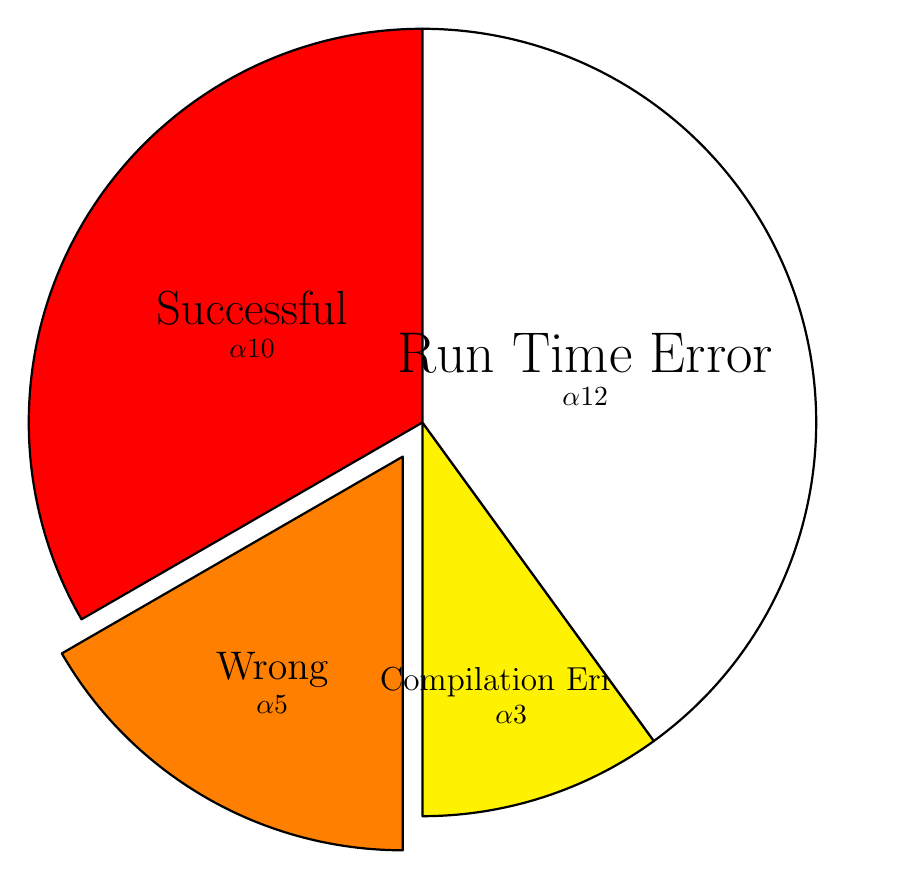
\begin{tikzpicture}
		\pie[before number={$\alpha$},rotate=90,pos={2,3},radius=5,explode = { 0, 0.5, 0,0},text=inside,color = {red, orange,yellow,white},sum=auto,scale font]{
			10/Successful, 5/Wrong, 3/Compilation Error, 12/Run Time Error
		}	
	\end{tikzpicture}
	
	\vspace{2cm}
		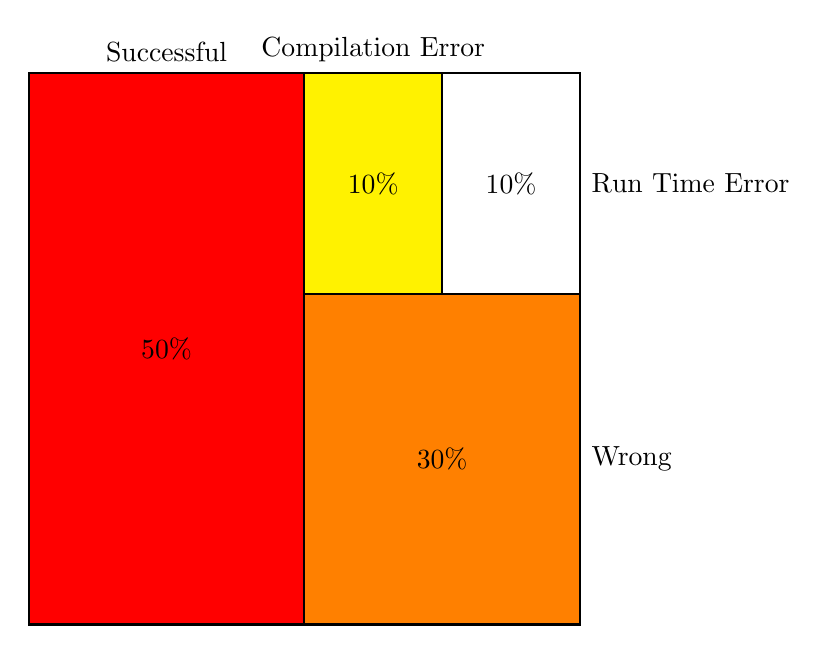
\begin{tikzpicture}
	\pie[square,rotate=180,explode = 0.1,color = {red, orange,yellow,white},radius = 3.5]{
		50/Successful, 30/Wrong, 10/Compilation Error, 10/Run Time Error
	}	
	\end{tikzpicture}
	
	\vspace{2cm}
	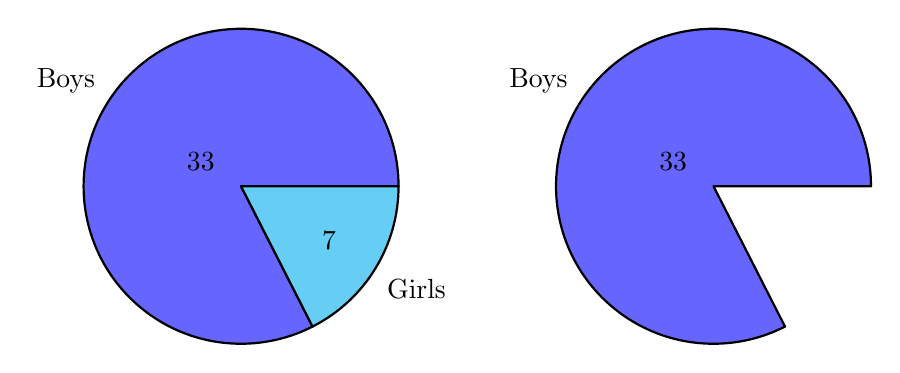
\begin{tikzpicture}
	\pie[ sum = auto , after number = , radius =2]{33/
		Boys , 7/ Girls }
	\pie[ pos ={6 ,0} , sum =40 , after number =, radius
	=2]{33/ Boys }
	\end{tikzpicture}\\
	\vspace{2cm}
	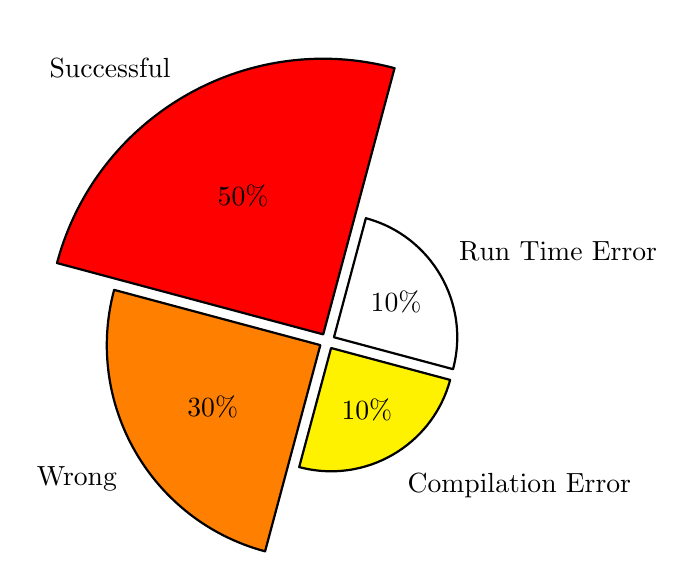
\begin{tikzpicture}
	\pie[polar,rotate=75,explode = 0.1,color = {red, orange,yellow,white},radius = 3.5]{
		50/Successful, 30/Wrong, 10/Compilation Error, 10/Run Time Error
	}	
	\end{tikzpicture}	

	\vspace{2cm}
	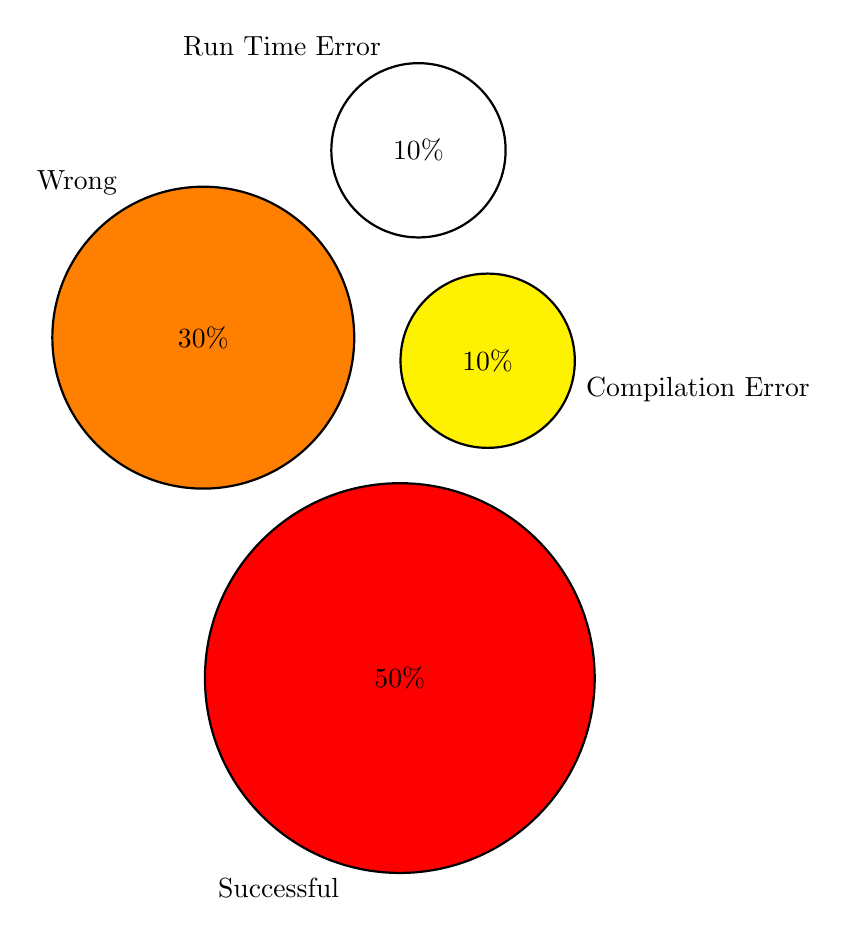
\begin{tikzpicture}
	\pie[cloud,rotate=75,explode = 0.5,color = {red, orange,yellow,white},radius = 3.5]{
		50/Successful, 30/Wrong, 10/Compilation Error, 10/Run Time Error
	}	
	\end{tikzpicture}
	
	\vspace{5cm}
	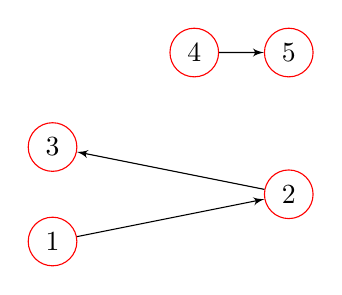
\begin{tikzpicture}
	[scale=.6,auto=center,every node/.style={circle,draw=red}]
	\tikzset{edge/.style = {->,> = latex'}}
	\node (n1) at (1,1) {1}; 
	\node (n2) at (6,2) {2};
	\node (n3) at (1,3) {3};
	\node (n4) at (4,5) {4};
	\node (n5) at (6,5) {5};
	
	\foreach \from/\to in {n1/n2,n2/n3,n4/n5}
	\draw[edge] (\from)--(\to);
	\end{tikzpicture}
	
	\vspace{5cm}


		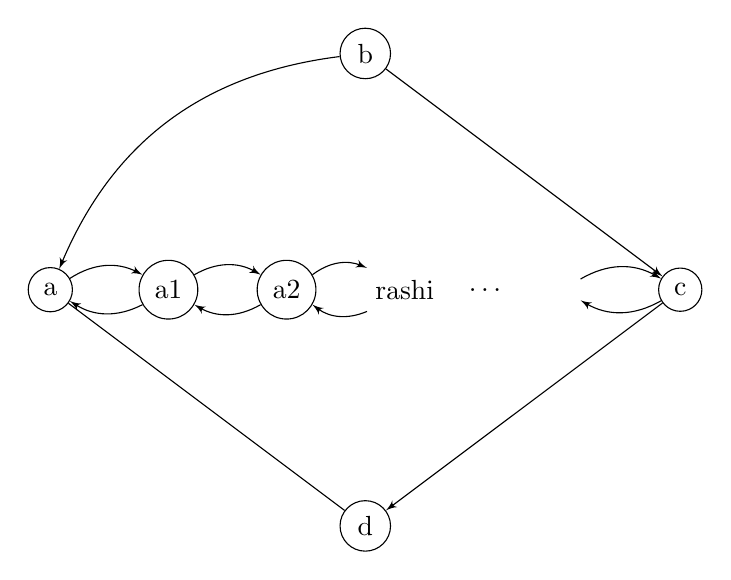
\begin{tikzpicture}
		
		\tikzset{vertex/.style = {shape=circle,draw,minimum size=1.5em}}
		\tikzset{edge/.style = {->,> = latex'}}
		% vertices
		\node[vertex] (a) at  (0,0) {a};
		\node[vertex] (b) at  (4,3) {b};
		\node[vertex] (c) at  (8,0) {c};
		\node[vertex] (d) at  (4,-3) {d};
		\node[vertex] (a1) at (1.5,0) {a1};
		\node[vertex] (a2) at (3,0) {a2};
		%edges
		\draw[edge] (b) to[bend right] (a);
		\draw[edge] (b) to (c);
		\draw (a) to (d); %undirected
		\draw[edge] (c) to (d);
		
		\draw[edge] (a)  to[bend left] (a1);
		\draw[edge] (a1) to[bend left] (a);
		
		\draw[edge] (a1) to[bend left] (a2);
		\draw[edge] (a2) to[bend left] (a1);
		
		\path (a2) to node {\dots} (c);
		\node [shape=circle,minimum size=1.5em] (a3) at (4.5,0) {rashi};
		\draw[edge] (a2) to[bend left] (a3);
		\draw[edge] (a3) to[bend left] (a2);
		%note that didn't use [vertex] which contains properties to make the circle
		
		\node [shape=circle,minimum size=1.5em] (c1) at (6.5,0) {};
		\draw[edge] (c) to[bend left] (c1);
		\draw[edge] (c1) to[bend left] (c);
		\end{tikzpicture}
		
		\vspace{5cm}
		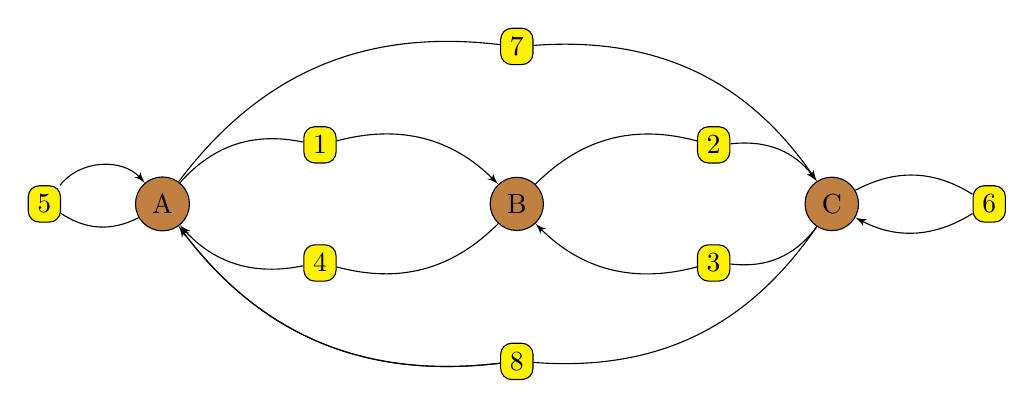
\begin{tikzpicture}
		
		\tikzset{vertex/.style = {shape=circle,fill=brown,draw,minimum size=1.5em}}
		\tikzset{vertex2/.style = {shape=rectangle,rounded corners,fill=yellow,draw}} 
		\tikzset{edge/.style = {->,> = latex'}}
		% vertices
		\node[vertex2] (5) at  (0,0) {5};
		\node[vertex2] (6) at  (12,0) {6};
		\node[vertex2] (7) at  (6,2) {7};
		\node[vertex2] (8) at  (6,-2) {8};
		\node[vertex2] (1) at  (3.5,0.75) {1};
		\node[vertex2] (4) at  (3.5,-0.75) {4};
		\node[vertex2] (2) at  (8.5,0.75) {2};
		\node[vertex2] (3) at  (8.5,-0.75) {3};
		\node[vertex] (A) at (1.5,0) {A};
		\node[vertex] (B) at (6,0) {B};
		\node[vertex] (C) at (10,0) {C};
		%edges
		\draw (A) to[bend left] (1); %undirected
		\draw (A) to[bend left] (7); %undirected
		\draw (C) to[bend left] (8); %undirected
		\draw (B) to[bend left] (4); %undirected
		\draw (B) to[bend left] (2); %undirected
		\draw (C) to[bend left] (3); %undirected
		\draw[edge] (7) to[bend left] (C);
		\draw[edge] (8) to[bend left] (A);
		\draw[edge] (1) to[bend left] (B);
		\draw[edge] (4) to[bend left] (A);
		\draw[edge] (2) to[bend left] (C);
		\draw[edge] (3) to[bend left] (B);
		\draw[edge] (8) to[bend left] (A);
		\draw[edge] (5) to[bend left=50] (A);
		\draw[edge] (6) to[bend left] (C);
		\draw (A) to[bend left] (5);
		\draw (C) to[bend left] (6);
		\end{tikzpicture}
	
	\vspace{5cm}
	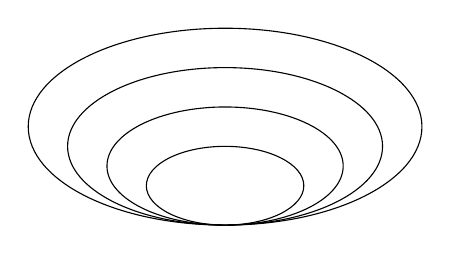
\begin{tikzpicture}
	\draw (0cm,0cm) ellipse[x radius=1cm,y radius=0.5cm];
	\draw (0cm,0.25cm) ellipse[x radius=1.5cm,y radius=0.75cm];
	\draw (0cm,0.5cm) ellipse[x radius=2cm,y radius=1cm];
	\draw (0cm,0.75cm) ellipse[x radius=2.5cm,y radius=1.25cm];
	\end{tikzpicture}
	
	\vspace{5cm}
	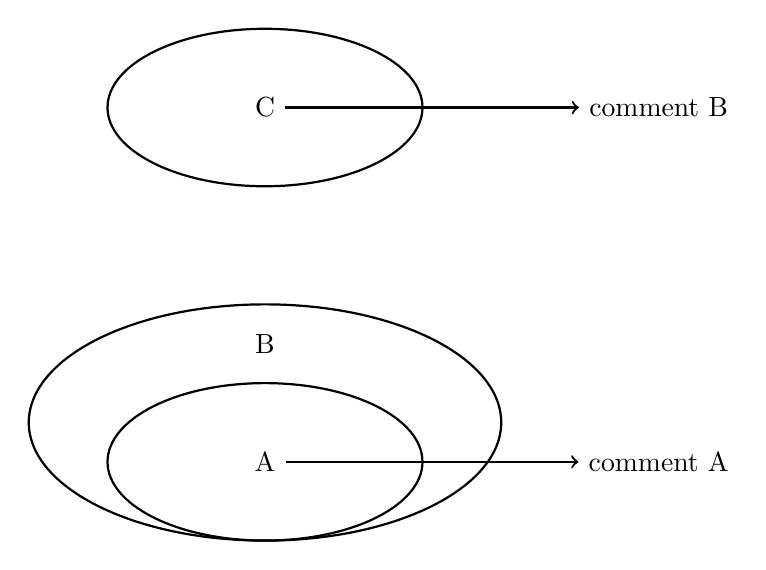
\begin{tikzpicture}[
	thick, scale=0.5]
	%\draw [help lines] (-3,-3) grid (3,3);
	\draw (0,1) ellipse(4 and 2) node(A){A};
	\draw (0,10) ellipse(4 and 2) node(C){C};
	\node (cB) at (10,10) {comment B};
	\draw [->] (C) -- (cB);
	\node (cA) at (10,1) {comment A};
	\draw [->] (A) -- (cA);
	\draw (0,2) ellipse(6 and 3) (0,4) node{B};
	\end{tikzpicture}
	\bibliographystyle{plainnat}
	\bibliography{bib}
\end{document}

